% Options for packages loaded elsewhere
\PassOptionsToPackage{unicode}{hyperref}
\PassOptionsToPackage{hyphens}{url}
\PassOptionsToPackage{dvipsnames,svgnames,x11names}{xcolor}
%
\documentclass[
  letterpaper,
  DIV=11,
  numbers=noendperiod]{scrreprt}

\usepackage{amsmath,amssymb}
\usepackage{lmodern}
\usepackage{iftex}
\ifPDFTeX
  \usepackage[T1]{fontenc}
  \usepackage[utf8]{inputenc}
  \usepackage{textcomp} % provide euro and other symbols
\else % if luatex or xetex
  \usepackage{unicode-math}
  \defaultfontfeatures{Scale=MatchLowercase}
  \defaultfontfeatures[\rmfamily]{Ligatures=TeX,Scale=1}
\fi
% Use upquote if available, for straight quotes in verbatim environments
\IfFileExists{upquote.sty}{\usepackage{upquote}}{}
\IfFileExists{microtype.sty}{% use microtype if available
  \usepackage[]{microtype}
  \UseMicrotypeSet[protrusion]{basicmath} % disable protrusion for tt fonts
}{}
\makeatletter
\@ifundefined{KOMAClassName}{% if non-KOMA class
  \IfFileExists{parskip.sty}{%
    \usepackage{parskip}
  }{% else
    \setlength{\parindent}{0pt}
    \setlength{\parskip}{6pt plus 2pt minus 1pt}}
}{% if KOMA class
  \KOMAoptions{parskip=half}}
\makeatother
\usepackage{xcolor}
\setlength{\emergencystretch}{3em} % prevent overfull lines
\setcounter{secnumdepth}{5}
% Make \paragraph and \subparagraph free-standing
\ifx\paragraph\undefined\else
  \let\oldparagraph\paragraph
  \renewcommand{\paragraph}[1]{\oldparagraph{#1}\mbox{}}
\fi
\ifx\subparagraph\undefined\else
  \let\oldsubparagraph\subparagraph
  \renewcommand{\subparagraph}[1]{\oldsubparagraph{#1}\mbox{}}
\fi

\usepackage{color}
\usepackage{fancyvrb}
\newcommand{\VerbBar}{|}
\newcommand{\VERB}{\Verb[commandchars=\\\{\}]}
\DefineVerbatimEnvironment{Highlighting}{Verbatim}{commandchars=\\\{\}}
% Add ',fontsize=\small' for more characters per line
\usepackage{framed}
\definecolor{shadecolor}{RGB}{241,243,245}
\newenvironment{Shaded}{\begin{snugshade}}{\end{snugshade}}
\newcommand{\AlertTok}[1]{\textcolor[rgb]{0.68,0.00,0.00}{#1}}
\newcommand{\AnnotationTok}[1]{\textcolor[rgb]{0.37,0.37,0.37}{#1}}
\newcommand{\AttributeTok}[1]{\textcolor[rgb]{0.40,0.45,0.13}{#1}}
\newcommand{\BaseNTok}[1]{\textcolor[rgb]{0.68,0.00,0.00}{#1}}
\newcommand{\BuiltInTok}[1]{\textcolor[rgb]{0.00,0.23,0.31}{#1}}
\newcommand{\CharTok}[1]{\textcolor[rgb]{0.13,0.47,0.30}{#1}}
\newcommand{\CommentTok}[1]{\textcolor[rgb]{0.37,0.37,0.37}{#1}}
\newcommand{\CommentVarTok}[1]{\textcolor[rgb]{0.37,0.37,0.37}{\textit{#1}}}
\newcommand{\ConstantTok}[1]{\textcolor[rgb]{0.56,0.35,0.01}{#1}}
\newcommand{\ControlFlowTok}[1]{\textcolor[rgb]{0.00,0.23,0.31}{#1}}
\newcommand{\DataTypeTok}[1]{\textcolor[rgb]{0.68,0.00,0.00}{#1}}
\newcommand{\DecValTok}[1]{\textcolor[rgb]{0.68,0.00,0.00}{#1}}
\newcommand{\DocumentationTok}[1]{\textcolor[rgb]{0.37,0.37,0.37}{\textit{#1}}}
\newcommand{\ErrorTok}[1]{\textcolor[rgb]{0.68,0.00,0.00}{#1}}
\newcommand{\ExtensionTok}[1]{\textcolor[rgb]{0.00,0.23,0.31}{#1}}
\newcommand{\FloatTok}[1]{\textcolor[rgb]{0.68,0.00,0.00}{#1}}
\newcommand{\FunctionTok}[1]{\textcolor[rgb]{0.28,0.35,0.67}{#1}}
\newcommand{\ImportTok}[1]{\textcolor[rgb]{0.00,0.46,0.62}{#1}}
\newcommand{\InformationTok}[1]{\textcolor[rgb]{0.37,0.37,0.37}{#1}}
\newcommand{\KeywordTok}[1]{\textcolor[rgb]{0.00,0.23,0.31}{#1}}
\newcommand{\NormalTok}[1]{\textcolor[rgb]{0.00,0.23,0.31}{#1}}
\newcommand{\OperatorTok}[1]{\textcolor[rgb]{0.37,0.37,0.37}{#1}}
\newcommand{\OtherTok}[1]{\textcolor[rgb]{0.00,0.23,0.31}{#1}}
\newcommand{\PreprocessorTok}[1]{\textcolor[rgb]{0.68,0.00,0.00}{#1}}
\newcommand{\RegionMarkerTok}[1]{\textcolor[rgb]{0.00,0.23,0.31}{#1}}
\newcommand{\SpecialCharTok}[1]{\textcolor[rgb]{0.37,0.37,0.37}{#1}}
\newcommand{\SpecialStringTok}[1]{\textcolor[rgb]{0.13,0.47,0.30}{#1}}
\newcommand{\StringTok}[1]{\textcolor[rgb]{0.13,0.47,0.30}{#1}}
\newcommand{\VariableTok}[1]{\textcolor[rgb]{0.07,0.07,0.07}{#1}}
\newcommand{\VerbatimStringTok}[1]{\textcolor[rgb]{0.13,0.47,0.30}{#1}}
\newcommand{\WarningTok}[1]{\textcolor[rgb]{0.37,0.37,0.37}{\textit{#1}}}

\providecommand{\tightlist}{%
  \setlength{\itemsep}{0pt}\setlength{\parskip}{0pt}}\usepackage{longtable,booktabs,array}
\usepackage{calc} % for calculating minipage widths
% Correct order of tables after \paragraph or \subparagraph
\usepackage{etoolbox}
\makeatletter
\patchcmd\longtable{\par}{\if@noskipsec\mbox{}\fi\par}{}{}
\makeatother
% Allow footnotes in longtable head/foot
\IfFileExists{footnotehyper.sty}{\usepackage{footnotehyper}}{\usepackage{footnote}}
\makesavenoteenv{longtable}
\usepackage{graphicx}
\makeatletter
\def\maxwidth{\ifdim\Gin@nat@width>\linewidth\linewidth\else\Gin@nat@width\fi}
\def\maxheight{\ifdim\Gin@nat@height>\textheight\textheight\else\Gin@nat@height\fi}
\makeatother
% Scale images if necessary, so that they will not overflow the page
% margins by default, and it is still possible to overwrite the defaults
% using explicit options in \includegraphics[width, height, ...]{}
\setkeys{Gin}{width=\maxwidth,height=\maxheight,keepaspectratio}
% Set default figure placement to htbp
\makeatletter
\def\fps@figure{htbp}
\makeatother
\newlength{\cslhangindent}
\setlength{\cslhangindent}{1.5em}
\newlength{\csllabelwidth}
\setlength{\csllabelwidth}{3em}
\newlength{\cslentryspacingunit} % times entry-spacing
\setlength{\cslentryspacingunit}{\parskip}
\newenvironment{CSLReferences}[2] % #1 hanging-ident, #2 entry spacing
 {% don't indent paragraphs
  \setlength{\parindent}{0pt}
  % turn on hanging indent if param 1 is 1
  \ifodd #1
  \let\oldpar\par
  \def\par{\hangindent=\cslhangindent\oldpar}
  \fi
  % set entry spacing
  \setlength{\parskip}{#2\cslentryspacingunit}
 }%
 {}
\usepackage{calc}
\newcommand{\CSLBlock}[1]{#1\hfill\break}
\newcommand{\CSLLeftMargin}[1]{\parbox[t]{\csllabelwidth}{#1}}
\newcommand{\CSLRightInline}[1]{\parbox[t]{\linewidth - \csllabelwidth}{#1}\break}
\newcommand{\CSLIndent}[1]{\hspace{\cslhangindent}#1}

\KOMAoption{captions}{tableheading}
\makeatletter
\@ifpackageloaded{tcolorbox}{}{\usepackage[many]{tcolorbox}}
\@ifpackageloaded{fontawesome5}{}{\usepackage{fontawesome5}}
\definecolor{quarto-callout-color}{HTML}{909090}
\definecolor{quarto-callout-note-color}{HTML}{0758E5}
\definecolor{quarto-callout-important-color}{HTML}{CC1914}
\definecolor{quarto-callout-warning-color}{HTML}{EB9113}
\definecolor{quarto-callout-tip-color}{HTML}{00A047}
\definecolor{quarto-callout-caution-color}{HTML}{FC5300}
\definecolor{quarto-callout-color-frame}{HTML}{acacac}
\definecolor{quarto-callout-note-color-frame}{HTML}{4582ec}
\definecolor{quarto-callout-important-color-frame}{HTML}{d9534f}
\definecolor{quarto-callout-warning-color-frame}{HTML}{f0ad4e}
\definecolor{quarto-callout-tip-color-frame}{HTML}{02b875}
\definecolor{quarto-callout-caution-color-frame}{HTML}{fd7e14}
\makeatother
\makeatletter
\makeatother
\makeatletter
\@ifpackageloaded{bookmark}{}{\usepackage{bookmark}}
\makeatother
\makeatletter
\@ifpackageloaded{caption}{}{\usepackage{caption}}
\AtBeginDocument{%
\ifdefined\contentsname
  \renewcommand*\contentsname{Table of contents}
\else
  \newcommand\contentsname{Table of contents}
\fi
\ifdefined\listfigurename
  \renewcommand*\listfigurename{List of Figures}
\else
  \newcommand\listfigurename{List of Figures}
\fi
\ifdefined\listtablename
  \renewcommand*\listtablename{List of Tables}
\else
  \newcommand\listtablename{List of Tables}
\fi
\ifdefined\figurename
  \renewcommand*\figurename{Figure}
\else
  \newcommand\figurename{Figure}
\fi
\ifdefined\tablename
  \renewcommand*\tablename{Table}
\else
  \newcommand\tablename{Table}
\fi
}
\@ifpackageloaded{float}{}{\usepackage{float}}
\floatstyle{ruled}
\@ifundefined{c@chapter}{\newfloat{codelisting}{h}{lop}}{\newfloat{codelisting}{h}{lop}[chapter]}
\floatname{codelisting}{Listing}
\newcommand*\listoflistings{\listof{codelisting}{List of Listings}}
\makeatother
\makeatletter
\@ifpackageloaded{caption}{}{\usepackage{caption}}
\@ifpackageloaded{subcaption}{}{\usepackage{subcaption}}
\makeatother
\makeatletter
\@ifpackageloaded{tcolorbox}{}{\usepackage[many]{tcolorbox}}
\makeatother
\makeatletter
\@ifundefined{shadecolor}{\definecolor{shadecolor}{rgb}{.97, .97, .97}}
\makeatother
\makeatletter
\makeatother
\ifLuaTeX
  \usepackage{selnolig}  % disable illegal ligatures
\fi
\IfFileExists{bookmark.sty}{\usepackage{bookmark}}{\usepackage{hyperref}}
\IfFileExists{xurl.sty}{\usepackage{xurl}}{} % add URL line breaks if available
\urlstyle{same} % disable monospaced font for URLs
\hypersetup{
  pdftitle={Basic Soil Science (SOIL 2125) Lab Manual - Spring 2023},
  pdfauthor={Nic Jelinski},
  colorlinks=true,
  linkcolor={blue},
  filecolor={Maroon},
  citecolor={Blue},
  urlcolor={Blue},
  pdfcreator={LaTeX via pandoc}}

\title{Basic Soil Science (SOIL 2125) Lab Manual - Spring 2023}
\author{Nic Jelinski}
\date{22DEC2022}

\begin{document}
\maketitle
\ifdefined\Shaded\renewenvironment{Shaded}{\begin{tcolorbox}[boxrule=0pt, interior hidden, enhanced, frame hidden, sharp corners, borderline west={3pt}{0pt}{shadecolor}, breakable]}{\end{tcolorbox}}\fi

\renewcommand*\contentsname{Table of contents}
{
\hypersetup{linkcolor=}
\setcounter{tocdepth}{2}
\tableofcontents
}
\bookmarksetup{startatroot}

\hypertarget{preface}{%
\chapter*{Preface}\label{preface}}
\addcontentsline{toc}{chapter}{Preface}

\begin{quote}
\hypertarget{tell-me-an-i-forget-teach-me-and-i-may-remember-involve-me-and-i-learn.}{%
\subsection*{\texorpdfstring{\textbf{``Tell me an I forget, teach me and
I may remember, involve me and I
learn.''}}{``Tell me an I forget, teach me and I may remember, involve me and I learn.''}}\label{tell-me-an-i-forget-teach-me-and-i-may-remember-involve-me-and-i-learn.}}
\addcontentsline{toc}{subsection}{\textbf{``Tell me an I forget, teach
me and I may remember, involve me and I learn.''}}

\hypertarget{benjamin-franklin}{%
\subsection*{\texorpdfstring{\emph{- Benjamin
Franklin}}{- Benjamin Franklin}}\label{benjamin-franklin}}
\addcontentsline{toc}{subsection}{\emph{- Benjamin Franklin}}
\end{quote}

\begin{tcolorbox}[enhanced jigsaw, opacityback=0, titlerule=0mm, bottomtitle=1mm, breakable, title=\textcolor{quarto-callout-note-color}{\faInfo}\hspace{0.5em}{Laboratory Schedule}, left=2mm, toptitle=1mm, opacitybacktitle=0.6, coltitle=black, arc=.35mm, leftrule=.75mm, colbacktitle=quarto-callout-note-color!10!white, rightrule=.15mm, toprule=.15mm, bottomrule=.15mm, colframe=quarto-callout-note-color-frame, colback=white]
Note that the laboratory portion of this course is self-paced. The lab
has open hours and is self-paced so you can return as often as needed to
complete the lab exercises (Laboratory TA's will be in the lab during
all open hours to help you). \textbf{Make sure you sign in and out}.

Labs take approximately 1-2 hrs to complete. You will sign up for a
timeslot of your choice. Open times: W 9:00 AM - 8:30 PM Th 9:00 AM -
8:30 PM F 9:00 AM - 4:30 PM \emph{241 Borlaug Hall}
\end{tcolorbox}

\hypertarget{lab-teaching-team}{%
\section*{Lab Teaching Team}\label{lab-teaching-team}}
\addcontentsline{toc}{section}{Lab Teaching Team}

\textbf{Teaching Support and Lab Coordinator}

Nora Pearson

pear0747@umn.edu

Office Hours (Zoom):

M 9:35-10:25AM, and by appointment

\textbf{Laboratory TAs}

XXXXX

XXXXX

\hypertarget{logitstics-and-laboratory-philosophy}{%
\section*{Logitstics and Laboratory
Philosophy}\label{logitstics-and-laboratory-philosophy}}
\addcontentsline{toc}{section}{Logitstics and Laboratory Philosophy}

\#\#\#Whys is this lab self-paced and what does that even mean?

Something here about pedagogy

\hypertarget{how-will-i-fit-the-lab-into-my-schedule}{%
\subsection*{How will I fit the lab into my
schedule?}\label{how-will-i-fit-the-lab-into-my-schedule}}
\addcontentsline{toc}{subsection}{How will I fit the lab into my
schedule?}

details here

\hypertarget{anything-else}{%
\subsection*{Anything else?}\label{anything-else}}
\addcontentsline{toc}{subsection}{Anything else?}

dunno

\bookmarksetup{startatroot}

\hypertarget{soil-texture-color-and-structure}{%
\chapter{\texorpdfstring{\textbf{Soil Texture, Color, and
Structure}}{Soil Texture, Color, and Structure}}\label{soil-texture-color-and-structure}}

\begin{tcolorbox}[enhanced jigsaw, opacityback=0, titlerule=0mm, bottomtitle=1mm, breakable, title=\textcolor{quarto-callout-note-color}{\faInfo}\hspace{0.5em}{Objectives}, left=2mm, toptitle=1mm, opacitybacktitle=0.6, coltitle=black, arc=.35mm, leftrule=.75mm, colbacktitle=quarto-callout-note-color!10!white, rightrule=.15mm, toprule=.15mm, bottomrule=.15mm, colframe=quarto-callout-note-color-frame, colback=white]

\begin{itemize}
\tightlist
\item
  Use the Bouyoucos hydrometer to determine soil particle distribution.
\item
  Use the textural triangle to determine the soil textural class name.
\item
  Use the texture by ``feel'' method to determine soil textural classes.
\item
  Determine soil color using Munsell notation.
\item
  Describe different soil structure characteristics and determine the
  horizon where most commonly found.
\end{itemize}

\end{tcolorbox}

\begin{tcolorbox}[enhanced jigsaw, opacityback=0, titlerule=0mm, bottomtitle=1mm, breakable, title=\textcolor{quarto-callout-tip-color}{\faLightbulb}\hspace{0.5em}{Key Words \& Concepts}, left=2mm, toptitle=1mm, opacitybacktitle=0.6, coltitle=black, arc=.35mm, leftrule=.75mm, colbacktitle=quarto-callout-tip-color!10!white, rightrule=.15mm, toprule=.15mm, bottomrule=.15mm, colframe=quarto-callout-tip-color-frame, colback=white]

\begin{itemize}
\tightlist
\item
  Blah Blah
\end{itemize}

\end{tcolorbox}

\hypertarget{investigation-a-using-a-hydrometer-to-determine-particle-size}{%
\section{INVESTIGATION A: Using a Hydrometer to Determine Particle
Size}\label{investigation-a-using-a-hydrometer-to-determine-particle-size}}

\hypertarget{theory}{%
\subsection{Theory}\label{theory}}

Particle size distribution has become a standard means for
characterizing and classifying the fine earth fraction of solid soil
particles, and is used to determine the soil texture class. This
experiment uses a Bouyoucos hydrometer to measure the density (grams per
L) of a liquid mixture (``slurry'') of soil and water.

Using the hydrometer allows us to determine soil texture by measuring
the grams of the soil particles (sand, silt, and, clay) that remain
suspended in the cylinder after a specific period of time. Different
sized soil particles are separated by their different sedimentation
rates -- e.g.~larger particles will settle faster in a column of water,
while smaller particles remain suspended much longer in the solution
(based on Stokes Law).

\begin{tcolorbox}[enhanced jigsaw, opacityback=0, titlerule=0mm, bottomtitle=1mm, breakable, title=\textcolor{quarto-callout-note-color}{\faInfo}\hspace{0.5em}{Watch this video before you start Investigation A}, left=2mm, toptitle=1mm, opacitybacktitle=0.6, coltitle=black, arc=.35mm, leftrule=.75mm, colbacktitle=quarto-callout-note-color!10!white, rightrule=.15mm, toprule=.15mm, bottomrule=.15mm, colframe=quarto-callout-note-color-frame, colback=white]


\includegraphics{./laboratory-1_files/figure-pdf/unnamed-chunk-1-1.pdf}

\end{tcolorbox}

\hypertarget{preparation}{%
\subsection{Preparation}\label{preparation}}

The two cylinders in this investigation each contain \textbf{\emph{60}}
grams of oven-dry dispersed soil -- one soil is from an E horizon and
one is from a B horizon. After mixing thoroughly with a stir stick, the
largest particles (sand) will quickly drop to the bottom of the
cylinder. After 40 seconds, only silt and clay particles are left
suspended in the water. After two hours only clay-sized particles
remain.

\hypertarget{measurements}{%
\subsection{Measurements}\label{measurements}}

\hypertarget{second-measurement}{%
\subsubsection{\texorpdfstring{\emph{40 Second
Measurement}}{40 Second Measurement}}\label{second-measurement}}

\begin{enumerate}
\def\labelenumi{\arabic{enumi}.}
\item
  Carefully use the stirring rod (approximately 18 inches long with a
  disk on the end) to completely disperse the soil in the cylinder. This
  requires that you \emph{slowly} lower and lift the stirring rod up and
  down in the cylinder until \textbf{\emph{all the sediment is removed
  from the bottom of the cylinder.}}
\item
  After stirring, immediately note the time to the nearest second.
  \emph{Carefully} and \emph{slowly} insert the hydrometer
  (\textbf{\emph{the hydrometers are extremely fragile}}) into the
  cylinder. Please refer to the figure on page 2. (\emph{Note}: you may
  need to use your finger to stop the hydrometer from bobbing).
\item
  After 40 seconds, read the number (at liquid level) on the hydrometer.
\item
  This reading must be corrected for temperature. Add 0.4 g/L for each
  degree above 20ºCelcius or subtract 0.4 g/L for each degree below
  20ºCelcius.
\end{enumerate}

\hypertarget{hour-measurement}{%
\subsubsection{\texorpdfstring{\emph{2 Hour
Measurement}}{2 Hour Measurement}}\label{hour-measurement}}

\begin{enumerate}
\def\labelenumi{\arabic{enumi}.}
\tightlist
\item
  Due to time constraints, two hour readings will be provided in lab.
\end{enumerate}

\begin{figure}

{\centering 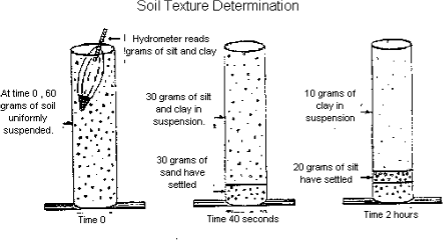
\includegraphics{./hydrometer-Picture1.png}

}

\caption{\label{fig-hydrometer}Hydrometer Process}

\end{figure}

(Note: The soil in the diagram has (60-30)/60 x 100= 50\% Sand; 10/60
x100= 17\% Clay; 100-50-17=33\% Silt)

\hypertarget{calculations---note-correct-readings-before-calculating-sand-silt-and-clay}{%
\subsubsection{\texorpdfstring{\emph{Calculations - note: correct
readings before calculating sand, silt, and
clay!}}{Calculations - note: correct readings before calculating sand, silt, and clay!}}\label{calculations---note-correct-readings-before-calculating-sand-silt-and-clay}}

\[
Sand (\%) = \frac{M_{sample,ovendry} - 40s reading}{M_{sample,ovendry}} x 100%
\]

\hypertarget{results}{%
\subsubsection{\texorpdfstring{\emph{Results}}{Results}}\label{results}}

\begin{longtable}[]{@{}lll@{}}
\toprule()
\textbf{Measurements} & \textbf{Sample 1} & \textbf{Sample 2} \\
\midrule()
\endhead
Sample mass (oven-dry) & 60g & 60g \\
40s reading (uncorrected) & g/L & g/L \\
Temperature (C) & C & C \\
40s reading (corrected) & g/L & g/L \\
\% Sand & \% & \% \\
2hr reading (uncorrected) & g/L & g/L \\
Temperature @ 2hr (C) & C & C \\
2hr reading (corrected) & g/L & g/L \\
\% Clay & \% & \% \\
\% Silt & \% & \% \\
\bottomrule()
\end{longtable}

\begin{longtable}[]{@{}lll@{}}
\toprule()
\textbf{Summary (copy values from above)} & \textbf{Sample 1} &
\textbf{Sample 2} \\
\midrule()
\endhead
Sand (\%) & & \\
Silt (\%) & & \\
Clay (\%) & & \\
\bottomrule()
\end{longtable}

\hypertarget{investigation-b-using-the-texture-triangle}{%
\section{INVESTIGATION B: Using the Texture
Triangle}\label{investigation-b-using-the-texture-triangle}}

\hypertarget{background}{%
\subsection{Background}\label{background}}

A soil's textural class is determined by that soil's respective content
of sand, silt, and clay. The USDA textural triangle is used to classify
the texture class of a soil. The sides of the soil textural triangle are
scaled for the percentages of sand, silt, and clay (0-100\%). Clay
percentages are read along the lines from left to right across the
triangle. Silt is read along the lines from the upper right to lower
left. Sand along the lines from lower right to the upper left portion of
the triangle. The intersections of the three sides on the triangle give
the texture class name. For instance, if you have a soil with 20\% clay,
45\% silt, and 35\% sand it falls in the ``loam'' textural class name.

\begin{figure}

{\centering 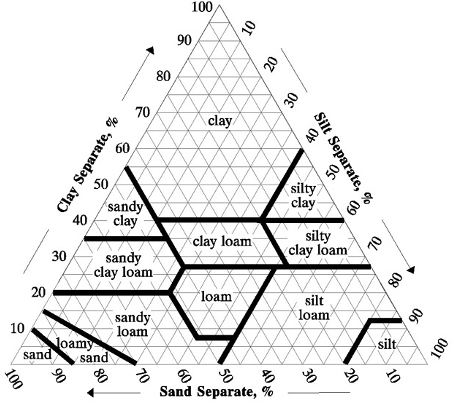
\includegraphics{./texture-triangle-Picture1.png}

}

\caption{\label{fig-triangle}USDA Soil Texture Triangle}

\end{figure}

\hypertarget{results-1}{%
\subsection{Results}\label{results-1}}

Using the soil particle percent data from Investigation A determine the
texture class for the soil samples 1 and 2.

\begin{longtable}[]{@{}
  >{\raggedright\arraybackslash}p{(\columnwidth - 8\tabcolsep) * \real{0.1644}}
  >{\raggedright\arraybackslash}p{(\columnwidth - 8\tabcolsep) * \real{0.1918}}
  >{\raggedright\arraybackslash}p{(\columnwidth - 8\tabcolsep) * \real{0.1918}}
  >{\raggedright\arraybackslash}p{(\columnwidth - 8\tabcolsep) * \real{0.1918}}
  >{\raggedright\arraybackslash}p{(\columnwidth - 8\tabcolsep) * \real{0.2603}}@{}}
\toprule()
\begin{minipage}[b]{\linewidth}\raggedright
\textbf{Sample}
\end{minipage} & \begin{minipage}[b]{\linewidth}\raggedright
\textbf{Sand (\%)}
\end{minipage} & \begin{minipage}[b]{\linewidth}\raggedright
\textbf{Silt (\%)}
\end{minipage} & \begin{minipage}[b]{\linewidth}\raggedright
\textbf{Clay (\%)}
\end{minipage} & \begin{minipage}[b]{\linewidth}\raggedright
\textbf{Texture Class}
\end{minipage} \\
\midrule()
\endhead
Sand (\%) & & & & \\
Silt (\%) & & & & \\
\bottomrule()
\end{longtable}

\bookmarksetup{startatroot}

\hypertarget{summary}{%
\chapter{Summary}\label{summary}}

In summary, this book has no content whatsoever.

\begin{Shaded}
\begin{Highlighting}[]
\DecValTok{1} \SpecialCharTok{+} \DecValTok{1}
\end{Highlighting}
\end{Shaded}

\begin{verbatim}
[1] 2
\end{verbatim}

\bookmarksetup{startatroot}

\hypertarget{references}{%
\chapter*{References}\label{references}}
\addcontentsline{toc}{chapter}{References}

\hypertarget{refs}{}
\begin{CSLReferences}{0}{0}
\end{CSLReferences}



\end{document}
